\documentclass[11pt]{article}
\usepackage[margin=1in]{geometry}
\usepackage{amsmath,amssymb}
\usepackage{booktabs}
\usepackage{graphicx}
\usepackage{tikz}
\usepackage{pgfplots}
\pgfplotsset{compat=1.17}
\usetikzlibrary{arrows.meta,positioning}
\usepackage[hidelinks]{hyperref}

\title{Exact instantiation of two achronal ANEC derivations: every evaluable display instance-confirmed on the instances that evaluated, except one verifier-gate gap}
\author{Gyalpo Dongo \and Sebastian Alberdi}
\date{18 September 2026}

\begin{document}
\maketitle

\begin{abstract}
The averaged null energy condition (ANEC) states that the null-null stress component, integrated along a complete null geodesic, is non-negative. Graham and Olum (2007) and Wall (2010) derive its achronal form through chains of displayed relations; Borde (1987) is the classical antecedent. We asked whether any derived display in these papers fails on an exact, premise-satisfying instance under the paper's own conventions and expansion order. We froze a registry of the displayed relations, classified each as premise, definition, imported result or derived relation, and built a mechanical verifier that evaluates a derived row in exact arithmetic, reporting a hit only when every printed premise holds and the relation fails. One search run explored 309 candidates. With one exception, every evaluable derived row of Graham and Olum and of Wall was exactly confirmed on every premise-satisfying instance that evaluated (a searcher-recorded outcome, not an engine count). The exception is Wall's equation (30): the ledger records one hit row on it, and the searcher's unreplayed sweep output (not on the ledger) holds four further instances of the family $R^{(1)}_{kk} = 8\pi T^{(1)}_{kk} + 1$ that the frozen predicate accepted. Inspection of the frozen evaluator shows that its equation-(30) branch omits the order-$\hbar$ Einstein identification $R^{(1)}_{kk} = 8\pi T^{(1)}_{kk}$ that the equation-(31) branch enforces; we classify the hit as a verifier defect by that inspection alone, pending a re-run under a repaired gate in an approved extension, and claim no error in Wall. The second hit row is the pre-registered calibration control on the Flanagan and Wald kernel constant, printed $12\pi$ in their Appendix D, Eqs.\ (D7) and (D13), and independently derived as $16\pi$. Neither frozen ship condition is met as written: no hit was re-verified by a source-based reimplementation, and no row carries a symbolic certificate. This is a partial question-status report shipped under a Director ruling, one status per paper: Graham and Olum instance-confirmed on every evaluated derived row; Wall parked on the non-evaluable rows W-23, W-26, W-32 and W-34 and on the equation-(30) gate gap; Borde parked, full text unavailable. The report carries instance-level confirmations for nine evaluable rows plus W-30 under a defective gate, named obstructions for the rest, and a geometry-versus-matter provenance for each step.
\end{abstract}

\section{Introduction}

Energy conditions are the inequalities on the stress tensor that singularity theorems, topological censorship and the exclusion of traversable wormholes consume. The averaged null energy condition (ANEC) is the weakest one still in wide use: for a complete null geodesic $\gamma$ with affine tangent $k^a$,
\begin{equation}
\int_\gamma T_{ab} k^a k^b \, d\lambda \;\ge\; 0 .
\label{eq:anec}
\end{equation}
Quantum fields violate the pointwise null energy condition, so the averaged form carries the exclusion arguments. Three papers anchor its status. Borde \cite{borde1987} proved focusing and singularity results from averaged conditions in the classical setting. Graham and Olum \cite{grahamolum2007} showed that ANEC can be violated along chronal geodesics by conformal rescaling and proposed the achronal restriction. Wall \cite{wall2010} derived the achronal ANEC from the generalized second law of horizon thermodynamics, working order by order in $\hbar$ around a classical background horizon.

These derivations are chains of displayed equations and inequalities. Each display is either a premise, a definition, an imported result, or a step derived from earlier displays. A derived display can be wrong in four ways that we name as mechanism families: a convention mismatch between the display and the text (F1), a finite algebraic slip such as a wrong coefficient (F2), an integration or limit that does not exist or changes sign (F3), and a premise used in a display that the text does not actually secure (F4). Readers rarely check every display, and a slip in one exclusion paper can propagate through the citation graph.

We asked one question. For each paper, does any derived display admit an exact, premise-satisfying instance on which the display fails, under the paper's printed conventions and expansion order? A positive answer would be a mechanically re-verified counterexample. A negative answer is a set of exact confirmations, one per row, plus a named obstruction for every row that cannot be evaluated mechanically. The contract for this campaign (Section~\ref{sec:protocol}) treats the second outcome as a first-class result. We report a partial version of it: the contract reserves the word \emph{certificate} for a symbolic closure, none was run, and neither frozen ship condition is met as written, so what we ship are instance-level confirmations and per-paper statuses under a Director ruling (Section~\ref{sec:hits}).

The resolution is this: Section~\ref{sec:confirm} reports that no evaluable derived row of either paper fails on any premise-satisfying instance, except W-30, where the frozen verifier accepts a family of instances because of a gap in its own premise gate; the two ledger hits are a calibration control and that verifier defect (Section~\ref{sec:hits}).

\section{Method}

\subsection{Row registry}
\label{sec:registry}

A \emph{row} is one displayed relation of one paper, read from the preprint bytes on 18 September 2026 (Graham and Olum arXiv:0705.3193v2, pages 2 to 4; Wall arXiv:0910.5751v2, pages 5 to 16). The registry is frozen inside the verifier and each row carries a kind: \emph{premise}, \emph{definition}, \emph{imported}, \emph{derived}, or \emph{prose}. Only derived rows are targets. The premise rows the evaluators gate on are W-5 (the Einstein equation $8\pi G\,T_{ab} = G_{ab}$ on the classical background, whose order-$\hbar$ bookkeeping W-12 gives $R^{(1)}_{kk} = 8\pi T^{(1)}_{kk}$), W-13 (horizon persistence: $\theta$ vanishes on both horizons through first order, so all half-order coefficients vanish), W-15 and W-16 (the generalized second law and its time reverse, the two generalized-entropy inequalities), W-23 (the unitarity identification of regions) and W-28 (the boundary conditions $\langle\theta_1\rangle \to 0$ at both ends of the geodesic). Definitions, premises and imported results are inputs, so a candidate can never redefine the object it is testing. Each row also records which quantities the step consumes: geometric curvature ($R_{ab}k^ak^b$), matter stress ($T_{ab}k^ak^b$), both, or neither. Table~\ref{tab:registry} lists the derived rows. In GO-5, $\Omega$ is the constant conformal factor, $a$ the trace-anomaly coefficient, $T_\gamma = \int_\gamma T_{ab}k^ak^b\,d\lambda$ and $J_\gamma$ the corresponding integral of the anomaly term $Z_{ab}k^ak^b$. The Graham and Olum registry has seven displays plus one prose note; the Wall registry has displays 4 through 34. Borde has no rows (Limitations).

\begin{table}[t]
\centering
\caption{Derived rows in the frozen registry. Ten carry a mechanical evaluator and are search targets. The others carry a named obstruction and abstain. The consumes column is the assumption-provenance map: which kind of quantity the step consumes.}
\label{tab:registry}
\small
\begin{tabular}{llll}
\toprule
Row & Relation (paper's notation) & Consumes & Evaluator \\
\midrule
GO-5 & $\int_\gamma T^a{}_b(\bar g)k^ak_b = \Omega^{-4}(T_\gamma - 8a\ln\Omega\, J_\gamma)$ & matter & exact, linear \\
W-7 & $-\dot\theta = \theta^2/2 + \sigma_{ab}\sigma^{ab} + 8\pi G\,T_{ab}k^ak^b$ & both & symbolic Ricci at a point \\
W-10 & order-$\hbar^0$ bookkeeping of $8\pi\langle T\rangle = \langle G\rangle$ & both & none (Director ruling) \\
W-11 & order-$\hbar^{1/2}$ bookkeeping & geometry & none (Director ruling) \\
W-12 & order-$\hbar^1$ bookkeeping & both & none (Director ruling) \\
W-17-18 & W-15 minus W-16 & none & exact, linear \\
W-23 & unitarity identification of regions & none & none (F4) \\
W-24 & rearrangement of W-23 & none & exact, linear \\
W-25 & entropy-area inequality & none & exact, linear \\
W-26 & $\langle\theta_{1,\mathrm{fut}}-\theta_{1,\mathrm{past}}\rangle \ge 0$ & none & none (interval quantifier, F4) \\
W-27 & $d\langle\theta_1\rangle/d\lambda = -8\pi\langle T_1\rangle_{kk}$ (gravitons ignored) & both & formal series in $\hbar^{1/2}$ \\
W-29 & $\int_X^\infty\langle T_1\rangle_{kk} + \int_{-\infty}^X\langle T_1\rangle_{kk} \ge 0$ & matter & ODE with W-28 \\
W-30 & $-d\langle\theta_1\rangle/d\lambda = \langle\sigma\sigma\rangle_1 + \langle R_{ab}\rangle_1 k^ak^b$ & geometry & formal series in $\hbar^{1/2}$ \\
W-31 & $-d\langle\theta_1\rangle/d\lambda = \langle\sigma\sigma\rangle_1 + 8\pi\langle T_1\rangle_{kk}$ & both & formal series in $\hbar^{1/2}$ \\
W-32 & W-26 restated under Wall's Section 7 premises & none & none (same obstruction as W-26) \\
W-33 & $\int(\langle T_1\rangle_{kk} + \langle\sigma\sigma\rangle_1/8\pi)\,d\lambda \ge 0$ & both & ODE with W-28 \\
W-34 & $N_s$ species sum with $N_s = \hbar^p$ & both & none (unquantified remainder, F3/F4) \\
\midrule
FW-D7 & kernel constant of $k^2\ln k^2$ printed as $12\pi$ (primary text, Appendix D, Eqs.\ (D7) and (D13)) & none & calibration control \\
FW-D7-corr. & same kernel, constant $16\pi$ & none & calibration control \\
\bottomrule
\end{tabular}
\end{table}

\subsection{Candidates and the verifier}

A candidate is a tuple $\{\text{paper}, \text{row}, \text{instance}, \text{conventions}\}$. The instance is exact data in the row's own family: rational or closed-form functions of the affine parameter for GO-5 and the series rows, a four-dimensional metric and tangent field as rational functions of the coordinates plus a rational point for W-7, rational entropy and area increments for the linear rows, and closed-form integrands with convergent line integrals for the ODE rows. Floats are refused.

The verifier's entry point \texttt{verify(candidate)} returns \texttt{valid=True} only when all of the following hold. The row exists, is derived, and has an evaluator. Any declared convention equals the pinned printed one: signature $(-,+,+,+)$, the Ricci sign convention of Misner, Thorne and Wheeler (MTW), $8\pi G\,T_{ab} = G_{ab}$ with $G = 1$ in Wall, affine null $k^a$, $\theta = \nabla_a k^a$, and an $\hbar$ expansion with half-integer orders. Every printed premise of the row is independently established on the instance: for GO-5, a constant positive $\Omega$ and convergent $T_\gamma$, $J_\gamma$; for W-7, a symmetric nondegenerate Lorentzian metric at the point, $k^a$ null and affinely geodesic as an identity, twist-free at the point, and $D = 4$; for the entropy rows, the W-15, W-16 and W-23 inequalities; for the series rows, $\theta_0 = \sigma_0 = T^{(0)}_{kk} = 0$ on the background horizon, no $\hbar^{1/2}$ terms consistent with W-13, W-7 satisfied as a formal identity through order $\hbar$, and Wall's Section 7 conjecture that the half-order terms do not separate, taken as a premise; for the ODE rows, convergence, the W-28 boundary conditions and the sign premise W-26/W-32. Then the printed relation, evaluated exactly at the printed order, fails: a nonzero residual or a violated inequality. Anything else is \texttt{valid=False} with a reason string. Exact confirmations return the reason \emph{exactly confirmed} and are audit artifacts, never hits. Rows with no evaluator abstain with the named missing operation.

For W-7 the candidate supplies geometry only. The verifier computes the Christoffel symbols, the Ricci tensor, $B_{ab} = \nabla_b k_a$, the expansion $\theta$, the shear $\sigma^2$, the twist $\omega^2$, $d\theta/d\lambda$, and $G_{ab}k^ak^b = R_{ab}k^ak^b$ at the point. A W-7 evaluation exceeding 5~s abstains and parks that route (contract).

\subsection{Calibration and rejection examples}

Two calibration rows exercise the verifier. Row FW-D7 records the position-space kernel constant of $k^2\ln k^2$ from Flanagan and Wald \cite{flanaganwald1996} as $12\pi$. The registry first transcribed that value from a secondary internal transcription (per the contract); the Director then pinned it from the primary preprint bytes (arXiv:gr-qc/9602052, Appendix D, Eqs.\ (D7) and (D13)), and the pin is recorded in the frozen verifier's header, so the contract's precondition for quoting the printed constant is satisfied. The verifier derives the constant independently as $2c'(2)$ from $c(\nu) = 2^{\nu+2}\pi\,\Gamma(1+\nu/2)/\Gamma(-\nu/2)$ through the reflection formula, obtaining $16\pi$, and cross-checks it with a numeric control on $h(r) = r^4 e^{-r^2}$ whose momentum integral divided by $\pi$ must equal $16\pi$. FW-D7 is therefore expected to hit and FW-D7-corrected (constant $16\pi$) is expected to confirm; the pair proves the verifier can distinguish a wrong constant from a right one. The contract further fixes five rejection examples that the frozen verifier must refuse: the planar Schwarzschild W-7 witness at $r=3$ (refused because W-7 is exactly confirmed on it), the FW-D7-corrected row, the definition GO-4, a W-29 instance that violates ANEC (an ANEC violator is a premise failure, never a counterexample to the derivation), and a W-7 instance declared in signature $(+,-,-,-)$. The engine confirmed all five refusals at freeze (ledger row \texttt{verifier\_premortem}).

\subsection{Harness protocol}
\label{sec:protocol}

The campaign ran inside an autoresearch harness in which every role is a disposable session and only the ledger carries state. An island is one searcher process with its own candidate stream; the Director is the human reviewer who freezes the contract and verifier; the engine is the harness code that writes ledger rows and derives counts from them. Figure~\ref{fig:pipeline} shows the loop. The pitch pre-registered the question, the mechanism families F1 to F4, the candidate templates and their order, and the kill criteria before any calculation. A search architect drafted the verifier. Three Director review rounds, recorded one minute apart with near-identical text, each reported the fixture suite failing on three W-7 fixtures of the original draft; a redraft repaired them and was frozen, and the Director later re-ran the fixture and witness suites on the frozen bytes with every fixture reporting ok (Limitations). The frozen file is hash-pinned on the ledger's reference row and the pin is checked before every run and before any hit row is written. The contract budget was one search run, one island, a 480~s clock, at most one symbolic closure plus 32 exact instantiations per row, and no cloud spend. A searcher session then explored candidates against the frozen verifier; it never sees any private battery and cannot edit the verifier. Every claimed hit and every near miss is a ledger row with the candidate, the verdict JSON and the environment hash. The engine derived every count in this paper from the ledger before the writer session was called; the writer session cites those counts and does not recount.

\begin{figure}[t]
\centering
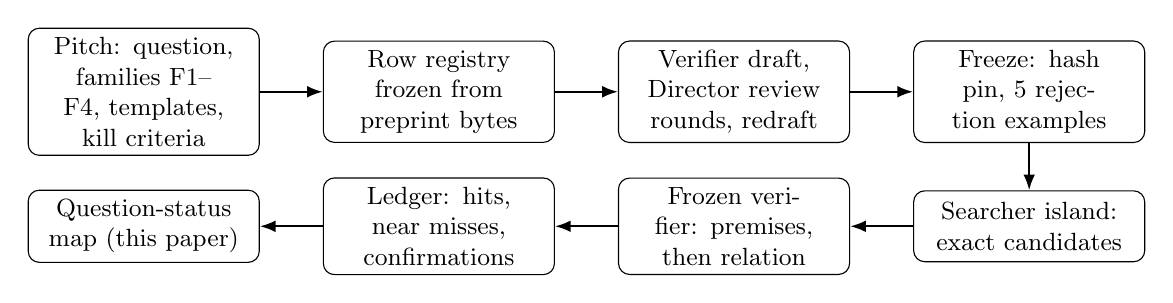
\begin{tikzpicture}[node distance=6mm and 8mm, box/.style={draw, rounded corners, align=center, minimum height=9mm, text width=27mm, font=\small}, arr/.style={-{Latex[length=2mm]}, thick}]
\node[box] (pitch) {Pitch: question, families F1--F4, templates, kill criteria};
\node[box, right=of pitch] (reg) {Row registry frozen from preprint bytes};
\node[box, right=of reg] (draft) {Verifier draft, Director review rounds, redraft};
\node[box, right=of draft] (freeze) {Freeze: hash pin, 5 rejection examples};
\node[box, below=of freeze] (search) {Searcher island: exact candidates};
\node[box, left=of search] (verify) {Frozen verifier: premises, then relation};
\node[box, left=of verify] (ledger) {Ledger: hits, near misses, confirmations};
\node[box, left=of ledger] (paper) {Question-status map (this paper)};
\draw[arr] (pitch) -- (reg);
\draw[arr] (reg) -- (draft);
\draw[arr] (draft) -- (freeze);
\draw[arr] (freeze) -- (search);
\draw[arr] (search) -- (verify);
\draw[arr] (verify) -- (ledger);
\draw[arr] (ledger) -- (paper);
\end{tikzpicture}
\caption{The campaign loop. Everything in the top row is fixed before the first candidate is evaluated. The searcher can propose candidates but cannot change the verifier; the writer reads only the ledger.}
\label{fig:pipeline}
\end{figure}

\section{Results}

\subsection{One run, 309 candidates, two hit rows}

Table~\ref{tab:census} is the engine-derived census. One run on one island explored 309 candidates and produced two hit rows, two distinct instances (by the verifier's own fingerprint: row plus canonicalized instance), zero duplicate rows, and four near-miss rows (candidates refused at a premise gate and recorded with the failed constraint and its margin). Figure~\ref{fig:census} plots the same numbers.

\begin{table}[t]
\centering
\caption{Search census (FACTS.json, engine-derived from the ledger).}
\label{tab:census}
\begin{tabular}{lrrrrr}
\toprule
Run & Islands & Explored & Hit rows & New instances & Near misses \\
\midrule
1 & 1 & 309 & 2 & 2 & 4 \\
\midrule
Total & 1 & 309 & 2 & 2 & 4 \\
\bottomrule
\end{tabular}
\end{table}

\begin{figure}[t]
\centering
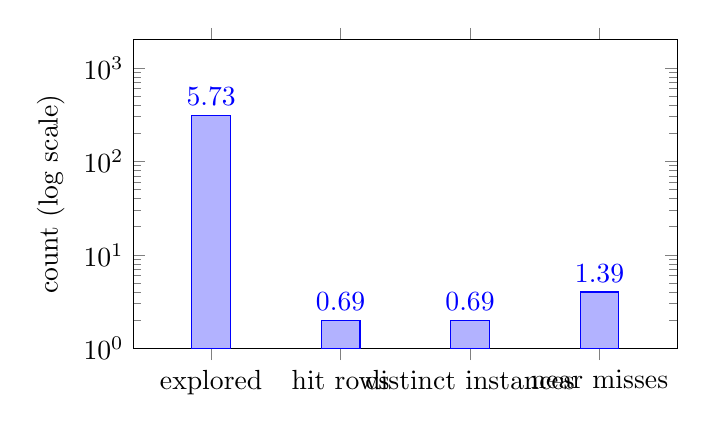
\begin{tikzpicture}
\begin{axis}[ybar, ymode=log, log origin=infty, width=0.7\textwidth, height=5.5cm, ylabel={count (log scale)}, symbolic x coords={explored, hit rows, distinct instances, near misses}, xtick=data, nodes near coords, nodes near coords align={vertical}, ymin=1, ymax=2000, bar width=14pt, enlarge x limits=0.2]
\addplot coordinates {(explored,309) (hit rows,2) (distinct instances,2) (near misses,4)};
\end{axis}
\end{tikzpicture}
\caption{Run-1 census; the two hit rows are explained in Section~\ref{sec:hits}.}
\label{fig:census}
\end{figure}

\subsection{Every evaluable row except W-30 is exactly confirmed on the instances that evaluated}
\label{sec:confirm}

The run-1 ledger row (SEARCH-1) records the dead ends in the searcher's own words: every evaluable derived row of Graham and Olum and of Wall was exactly confirmed on every premise-satisfying instance that evaluated. The same ledger field continues: the only \texttt{valid=True} on a target paper is the W-30 premise-gate gap, which is a verifier defect, not a paper defect. That sentence is the searcher's self-report, not an engine count, and no mechanical replay of the sweep is on the ledger, so the confirmation statement carries the searcher-recorded label throughout. The searcher's unreplayed sweep output (\texttt{workspace/out/results.json}, listed in FACTS.json, not on the ledger) records four premise-satisfying W-30 instances of the family $R^{(1)}_{kk} = 8\pi T^{(1)}_{kk} + 1$ returned \texttt{valid=True} with residual $-1$, of which the searcher claimed one hand-simplified representative as hit 0 (Section~\ref{sec:hits}). The families it reports are listed in Table~\ref{tab:families}. GO-5 is linear in $T_{kk}$ and $Z_{kk}$ with constant $\Omega$, so every instance is confirmed with zero residual. W-7 was confirmed on the reported rational geometries, including planar Schwarzschild outside the horizon, Reissner--Nordstr\"om, de Sitter and anti-de Sitter, Schwarzschild--de Sitter, flat space, power-law Friedmann--Robertson--Walker (FRW) cosmologies, a Bianchi diagonal metric, ingoing Eddington--Finkelstein and Vaidya. The three plane-fronted (pp) wave candidates were refused because their supplied tangent was not null; they are the three non-null refusals of Table~\ref{tab:families}, which the ledger's run row misattributes to the Eddington--Finkelstein tangents (those were confirmed). No pp-wave instance evaluated W-7. In each confirmed W-7 case the Raychaudhuri identity and the step $G_{ab}k^ak^b = R_{ab}k^ak^b$ were confirmed independently. The verifier's transcript for the rejection-example witness (planar Schwarzschild at $r=3$) reports $\theta = 2/3$, $d\theta/d\lambda = -2/9$, $\sigma^2 = 0$ and $R_{kk} = 0$. The linear rows W-17-18, W-24 and W-25 confirmed on every premise-satisfying grid point. The series rows W-27 and W-31 are not a grid: coverage is sparse (Table~\ref{tab:families}), most candidates were refused as malformed, W-27 also had premise refusals not recorded on the ledger, and the few candidates that evaluated confirmed. The ODE rows W-29 and W-33 confirmed on every candidate that evaluated; the ones that did not evaluate are the abstentions of Section~\ref{sec:near}.

\begin{table}[t]
\centering
\caption{Instance families explored in run 1, as recorded by the searcher in the run-1 ledger row (SEARCH-1). These counts are the searcher's record and were not recomputed by the engine.}
\label{tab:families}
\small
\begin{tabular}{lll}
\toprule
Row(s) & Family & Searcher-recorded outcome \\
\midrule
GO-5 & $\Omega\in\{2,3/2,1/3,e,7\}$, $a\in\{1/(2880\pi^2),-1/7,1/(8\pi),3\}$, closed-form $T_{kk}$, $Z_{kk}$ & 32 of 32 exactly confirmed \\
W-7 & rational geometries & 27 confirmed; 3 non-null tangents refused; 1 non-affine probe refused (the searcher's family total disagrees with this split and is not quoted; its recorded maximum evaluation time and the sweep output's maximum disagree with each other, both lying under the contract's 5~s park bound) \\
W-17-18, W-24, W-25 & rational grid in $\{-2,\dots,2\}$ & all premise-satisfying points confirmed \\
W-27, W-30, W-31 & formal series data & sparse coverage: most W-30 and W-31 candidates were refused as malformed (a parser gap on the tokens erf and atan) and never evaluated; the evaluated W-31 and W-27 candidates confirmed; the evaluated W-30 candidates split between confirmations and the $R^{(1)}_{kk} = 8\pi T^{(1)}_{kk} + 1$ family accepted by the defective gate of Section~\ref{sec:hits}; no per-row evaluated/abstained/malformed split is on the ledger \\
W-29, W-33 & closed-form integrands & 20 of 44 evaluated, all 20 confirmed; 24 abstained \\
\bottomrule
\end{tabular}
\end{table}

\subsection{Both hit rows are explained without a paper defect}
\label{sec:hits}

Table~\ref{tab:hits} reproduces the two verdict JSONs. Both carry \texttt{valid=True} and both are explained without a defect in a target paper.

\begin{table}[t]
\centering
\caption{Hit rows in the ledger, digit for digit from the verdict JSONs (SEARCH-1, hit index 0 and 1).}
\label{tab:hits}
\small
\begin{tabular}{llll}
\toprule
Hit & Row & Instance & Verdict metrics \\
\midrule
0 & W-30 & $\theta_1 = 0$, $T^{(1)}_{kk} = 0$, $\sigma^2_1 = 0$, $R^{(1)}_{kk} = 1$ & residual $-1$; consumes geometry \\
1 & FW-D7 & (none) & kernel constant $16\pi$; printed $12\pi$ (primary text, Eqs.\ (D7), (D13)); residual $4\pi$; \\
 & & & momentum integral over $\pi$ = 50.26548245743669181540229; \\
 & & & absolute deviation from $16\pi$ = $6.3109\times 10^{-30}$ \\
\bottomrule
\end{tabular}
\end{table}

\paragraph{Hit 1 is the calibration control.} FW-D7 is not a target paper row. The contract pre-registered it as the positive control that must hit, and FW-D7-corrected as the matching control that must confirm; the premortem row records the latter refusal with the reason \emph{independent kernel constant $2c'(2) = 16\pi$}. The pair behaved as pre-registered. The $12\pi$ entered the registry as a secondary transcription and was afterwards pinned to the primary text (Appendix D, Eqs.\ (D7) and (D13); Section 2.3), which is what the contract requires before a calibration claim leaves the harness. The $16\pi$ derivation is the verifier's own self-test of that constant; it rests on the verifier's derivation, its numeric control and the internal transcription of Section 2.3, and has no external literature confirmation (no erratum search was run). This paper makes no further claim about Flanagan and Wald's argument.

\paragraph{Hit 0 is a verifier defect.} The instance sets every matter and expansion coefficient to zero and supplies $R^{(1)}_{kk} = 1$ as an independent datum. Reading the frozen evaluator explains why it is admitted. The premise gate for the series rows checks that W-7 holds as a formal identity through order $\hbar$ with $8\pi T_{kk}$ on the right-hand side; with all of $\theta_1$, $T^{(1)}_{kk}$ and $\sigma^2_1$ zero, that identity holds trivially. The W-30 branch then compares $-d\theta_1/d\lambda$ with $\sigma^2_1 + R^{(1)}_{kk}$ using the supplied $R^{(1)}_{kk}$, and the residual is $-1$. The W-31 branch, by contrast, first checks the order-$\hbar$ Einstein identification $R^{(1)}_{kk} = 8\pi T^{(1)}_{kk}$ (rows W-5 and W-12) and refuses the same data as a premise failure. The ledger records exactly this asymmetry, though not on the same data: near-miss row 1 is a different instance of the same family ($\theta_1 = -8\pi\lambda$, $T^{(1)}_{kk} = 1$, $\sigma^2_1 = 0$, $R^{(1)}_{kk} = 8\pi + 1$), with the same margin $R_1 - 8\pi T_1 = 1$, offered to W-31 and refused with the failed constraint \emph{premise W-5/W-12 gated by the W-31 evaluator}. The ledger's free-text field for that row calls it an identical instance to the W-30 hit; that wording is the searcher's error, since the two instances differ in every coefficient, and this paper follows the recorded candidate data rather than the prose. The searcher's unreplayed sweep output shows the same pairing for that instance and its siblings: the four instances of the family are accepted by W-30 and refused by W-31 at W-5/W-12, while their four siblings without a supplied $R^{(1)}_{kk}$ confirm with residual $0$; that with-versus-without pairing is a cheap counter-experiment supporting the gate-gap classification, though it is not on the ledger. The hit-0 instance itself ($\{0,0,0,1\}$) does not appear in the sweep output; it is the searcher's hand-simplified representative, re-verified by the engine at claim time. In Wall's text the curvature entering equation (30) is the semiclassical curvature of the perturbed metric, related to the stress tensor by the order-$\hbar$ Einstein equation of Wall's Section 3; an $R^{(1)}_{kk}$ decoupled from $T^{(1)}_{kk}$ is outside the paper's premises. The W-30 evaluator omits that gate. The searcher stated this doubt in its strategy field at the time of the claim. We therefore classify hit 0 as a premise-gate gap in the frozen verifier and claim no counterexample to Wall.

Neither of the contract's frozen ship conditions is met as written. Condition (a) requires a hit to be re-verified by a fresh source-based reimplementation; that reimplementation was not run, so (a) fails for hit 0 even before the classification above. Condition (b) requires all three papers CLOSED or PARKED with per-row certificates or obstructions, and the kill criteria say that instantiation agreement never substitutes for a symbolic certificate; no closure was run and W-30 remains an unresolved derived row, so (b) fails too. The paper therefore ships as a partial question-status report under a Director ruling (journal, 18 September 2026), with one status per paper. Graham and Olum: instance-confirmed on every evaluated derived row, no symbolic certificate. Wall: PARKED, on the non-evaluable rows W-23, W-26, W-32 and W-34 and on the W-30 premise-gate gap, whose classification above is by inspection of the frozen evaluator pending an approved extension that re-runs hit 0 under a repaired W-5/W-12 gate. Borde: PARKED, acquisition-gated. The W-30 gate repair and the per-row symbolic certificates are priced successor work, not part of this paper.

\subsection{Near misses are gates refusing correctly}
\label{sec:near}

Table~\ref{tab:near} lists the four near-miss rows. Each one records either a premise gate refusing correctly or an evaluator that could not evaluate; none is a relation failure.

\begin{table}[t]
\centering
\caption{Near-miss rows (SEARCH-1). Failed constraint and margin are quoted from the ledger.}
\label{tab:near}
\small
\begin{tabular}{llp{6.6cm}}
\toprule
Row & Failed constraint & Why it matters \\
\midrule
W-31 & premise W-5/W-12 ($R^{(1)}_{kk} = 8\pi T^{(1)}_{kk}$); margin $R_1 - 8\pi T_1 = 1$ & An instance with the same W-5/W-12 margin as hit 0 (not the same data); the refusal here is the whole content of hit 0. \\
W-27 & premise W-13: $\theta_{1/2}$ must be constant and vanish at both ends & Constant $\theta_{1/2} = 1$ passes constancy, fails the limits; the half-order gate is enforced. \\
W-7 & $k^b\nabla_b k^a = 0$ (non-affine rescaling of the witness tangent) & The affine gate rejects a rescaled null geodesic; W-7 cannot be broken by a parametrization choice (F1/F4 closed for this route). \\
W-33 & abstain: half-line integral unevaluated by the computer algebra system & Full-line integral converges but the half-line closed form is missing for several integrands; a coverage gap of the ODE evaluator, with 24 of 44 ODE candidates abstaining this way (searcher-recorded). \\
\bottomrule
\end{tabular}
\end{table}

\subsection{Assumption provenance and applicability findings}

The consumes column of Table~\ref{tab:registry} is the answer to the second half of the campaign question: which steps consume geometric curvature and which consume matter stress. In Graham and Olum the derived row GO-5 consumes matter only; the geometry enters through the definitions GO-4 and GO-7. In Wall the Raychaudhuri step W-7 and the series steps W-27, W-31 and W-33 consume both, W-30 consumes geometry only, W-29 consumes matter only, and the entropy rows W-17-18, W-24 and W-25 consume neither. The point where curvature is traded for stress is the pair W-30 to W-31, through W-5 and W-12; that is the gate hit 0 exposed (Section~\ref{sec:hits}).

The contract records two applicability findings; neither is a hit. First, W-7 prints the $D = 4$ coefficient $1/2$ on $\theta^2$ while the dimension is not printed; footnote 9 of Wall contemplates extra dimensions. There is no downstream consequence, because the relation is used at $\theta = \sigma = 0$ and linearized. Second, the prose note GO-P1 says $\Omega$ is of order $\exp(2880\pi^2)$, while the paper's own GO-5 with $T_\gamma \sim J_\gamma$ gives $\ln\Omega = 1/(8a) = 360\pi^2$; the logarithms differ by a factor of $8$; the prose is order-of-magnitude and has no consequence.

\section{Discussion}

The evaluable derived displays in Graham and Olum and in Wall are identities or linear consequences of their premises, and the contract predicted that the search on them would be a verifier exercise with a null result. That is what happened, with the W-30 gate gap as the one exception. The value of the run is the set of instance-level confirmations and the map of which rows can be checked mechanically, which cannot, and why. The contract's symbolic-closure budget (one closure per row) was not spent, so no row carries a certificate in the contract's sense, and W-30 cannot carry one while the frozen predicate accepts a family of its instances; that is why the report is partial (Section~\ref{sec:hits}).

The derived rows without an evaluator are the rows the method cannot yet reach. W-23 identifies regions by unitarity, W-26 and W-32 carry an interval quantifier with an implicit continuity assumption, and W-34 has an unquantified inter-sector remainder. Each needs a Director ruling on what the mechanical statement is before it can be a target; the contract parks Wall on those rows rather than letting an evaluator invent the statement. W-10 to W-12 are order-by-order bookkeeping of the semiclassical Einstein equation and need a ruling on whether they count as derived rows at all.

The hit-0 episode is a useful failure of the method. A verifier that gates premises row by row can carry a gap in one row's gate that its neighbour does not, and an exact search can find that gap. The fix is surgical: add the W-5/W-12 identification to the W-30 premise gate, or make the series premise check use the supplied $R^{(1)}_{kk}$ in the W-7 identity instead of $8\pi T^{(1)}_{kk}$. Either change moves the verifier hash and must go through an approved extension of the search, after which hit 0 should become an exact confirmation.

The calibration pair worked as designed and gives a template for future display audits: a row with a known wrong constant that must hit, next to the corrected row that must confirm, run in the same sweep as the targets.

\section{Limitations}

Borde \cite{borde1987} has no rows in the registry because only its abstract was accessible; nothing in this paper bears on that paper beyond parking it. The registry for Graham and Olum and Wall was transcribed from the preprint bytes by a harness session, and a transcription error in a row's text would propagate into its confirmations. No symbolic closure was run for any row, so every confirmation in this paper is instance-level and none is a certificate in the contract's sense. The ODE evaluator abstained on the candidates whose half-line antiderivative the computer algebra system could not close, so the W-29 and W-33 confirmations cover the evaluated candidates only. The W-7 confirmations cover the reported rational geometries at single rational points; they are not a symbolic closure over all metrics, although the relation is a textbook identity. The searcher's sweep output holds every candidate verdict and would allow the searcher-recorded outcomes of Table~\ref{tab:families} to be replayed mechanically; that replay is not on the ledger. The contract's kill criterion required the Director to run the fixture and witness suites, including the W-7 coefficient-discrimination control, before setup. The chronology on file is this: the three review rounds each recorded the fixture suite failing on three W-7 fixtures of the original draft (the signature classifier misclassified the planar witness, the non-null-tangent fixture never reached its premise, and the coefficient-discrimination control returned a null residual); the redraft that followed reported every fixture passing in its own changelog and was frozen one minute later; no passing run was recorded on the ledger before the freeze, and the verdict JSONs still carry the draft's own label that it was not machine-run by its drafter. After the critic audit, the Director re-ran the fixture and witness suites on the frozen verifier bytes and recorded the output (journal entry of 18 September 2026; log at \texttt{workspace/out/}): every fixture reported ok, the coefficient-discrimination control detected the wrong coefficient with residual $-2/9$, the planar witness confirmed as a non-hit, and the FW-D7 pair behaved as pre-registered. The W-7 confirmations therefore rest on an evaluator whose negative control passed on the frozen bytes, recorded after the run rather than before it. Finally, the run's ledger environment blocks record a newer Python interpreter than the contract's pinned python3.12, and the sympy and mpmath versions actually loaded are not attested on the ledger; the harness drift check reports no drift, so the run is internally consistent, but the reproduction pin below is the contract's, not the run's.

\section{Code availability}

The reproduction package was built locally (\texttt{campaigns/exclusion-display-audit/repro}) and, at the time of writing, is not yet published; it will be published at \texttt{github.com/oharalabsai/exclusion-display-audit-repro} after a clean-clone test. It contains the frozen contract, the frozen verifier with its row registry and calibration rows, every scored candidate with its verdict, the near-miss rows, the ledger, and a one-command reproduction script with the contract's pinned requirements (Python 3.12, sympy 1.14.0, mpmath 1.3.0; see Limitations for the interpreter the run actually recorded). The script asserts that every ledger hit still returns \texttt{valid=True} under the frozen predicate, which includes hit 0: reproducing the verifier defect is part of reproducing the result. No external dataset enters the campaign; every candidate is exact symbolic data. The symbolic engine is SymPy \cite{sympy2017}; mpmath is used for the numeric control only and never decides a verdict.

\section{AI-contribution statement}

The authors are responsible for every claim in this paper. An AI research harness executed the mechanical steps under human direction: transcribing the row registry from the preprints, drafting the verifier that the human Director reviewed and froze, enumerating candidates, and drafting this text from the ledger. Every number reported is a sealed-verifier verdict, an engine-derived count, or a searcher-recorded count quoted from the ledger and labelled as such, and the human authors reviewed the classification of both hit rows. No AI system is an author.

\bibliographystyle{unsrt}
\bibliography{references}

\end{document}
